\section{APPENDIX: MC closure Check}
\label{sec:MCclosureCheck}

To perform the MC closure check, the pseudodata samples are prepared to mimic each of the data samples needed for the fit. This includes:
\begin{itemize}
  \item $W\gamma$-selected samples to be used for fit (full analysis selection without $I_{ch}$ or $\sigma_{i\eta i\eta}$ cuts), those samples are prepared separately for the muon and electron channels;
  \item $W\gamma$ in full selection to be plotted into the [data vs bkg+signal] plots, separately for the two channels;
  \item $Z\gamma\rightarrow\mu\mu\gamma$ FSR selected sample for the real-$\gamma$ templates;
  \item $Z\gamma\rightarrow\mu\mu\gamma$ + (DY+jets) ISR selected sample for the fake-$\gamma$ templates.
\end{itemize}

To prepare the pseudodata $W\gamma$-selected samples, the $W\gamma$, $W$+jets, $Z\gamma$, DY+jets, $t\bar{t}\gamma$, $t\bar{t}$+jets, and $WW\gamma$ MC samples are merged with the $W\gamma$ selection applied. To prepare the pseudodata $Z\gamma$-selected samples, the $Z\gamma$ and DY+jets MC samples are merged with the appropriate $Z\gamma$ selections applied. Luminosity normalizations, PU and scale factor weights are applied on all MC samples. Then the pseudodata are treated as if they were data to perform the fits, prepare the plots and subtract the background. All the MC samples used in the nominal $W\gamma$ measurement are used for this MC closure check the same way.

Each of Fig.~\ref{fig:DATAvsBKGandSIGMC_MCclosure_MUON_B}-\ref{fig:DATAvsBKGandSIGMC_MCclosure_ELECTRON_E} consists of six plots. Three top plots are results of the event selection and background estimation in data while three bottom plots are results of the MC closure check. Left column is data (pseudodata) superimposed with MC. Since pseudodata is prepared as a mixture of MC samples, there is an exact match in pseudodata vs MC plots by construction. Middle and right plots show data vs background estimates and signal MC where jets$\rightarrow\gamma$ background is estimated from fits of $I_{ch}^{\gamma}$ (middle) and  $\sigma_{i\eta i\eta}^{\gamma}$ (right) templates.

\begin{figure}[htb]
  \begin{center}
   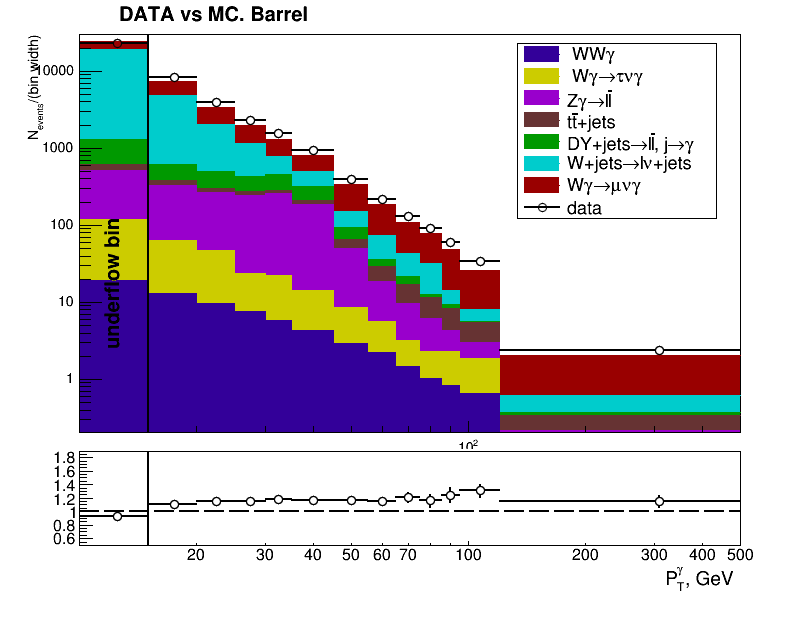
\includegraphics[width=0.33\textwidth]{../figs/figs_v11/MUON_WGamma/PrepareYields/c_TotalDATAvsMC_Barrel__phoEt.png}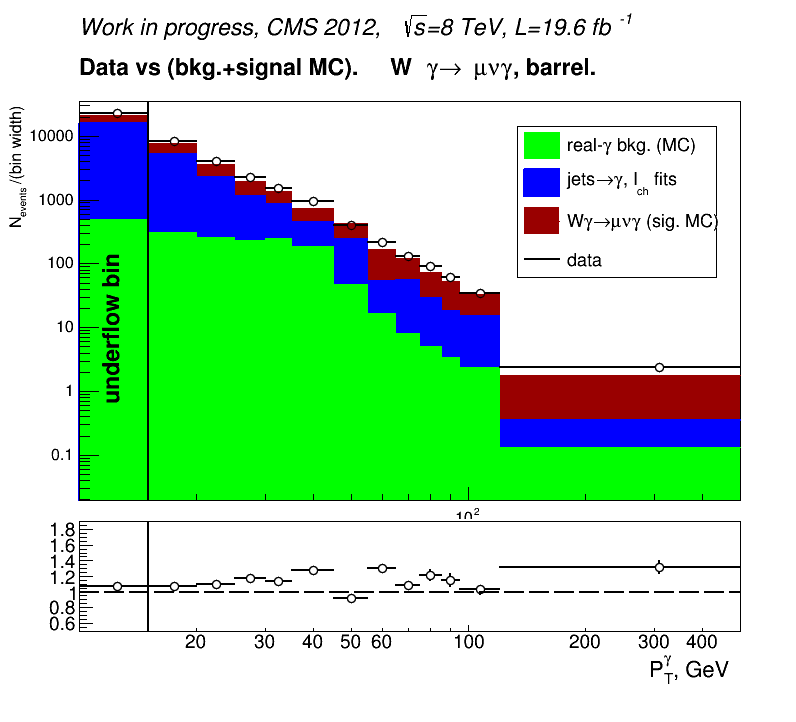
\includegraphics[width=0.33\textwidth]{../figs/figs_v11/MUON_WGamma/PrepareYields/c_DATAvsBkgPlusSigMCc_MUON_WGamma_TEMPL_CHISO_UNblind__Barrel__phoEt.png}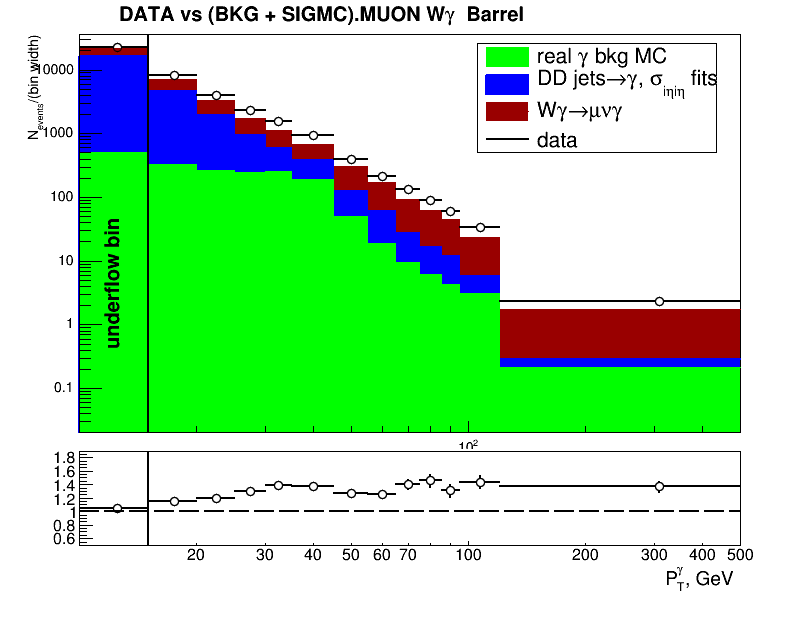
\includegraphics[width=0.33\textwidth]{../figs/figs_v11/MUON_WGamma/PrepareYields/c_DATAvsBkgPlusSigMCc_MUON_WGamma_TEMPL_SIHIH_UNblind__Barrel__phoEt.png}
   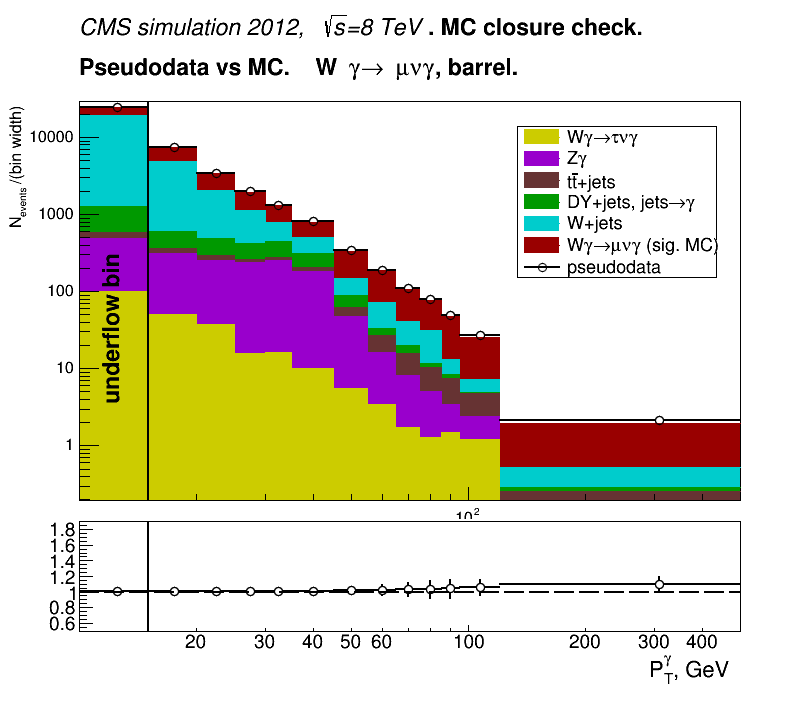
\includegraphics[width=0.33\textwidth]{../figs/figs_v11/MUON_WGamma/PrepareYields/c_TotalDATAvsMC_Barrel__phoEt_MCclosure.png}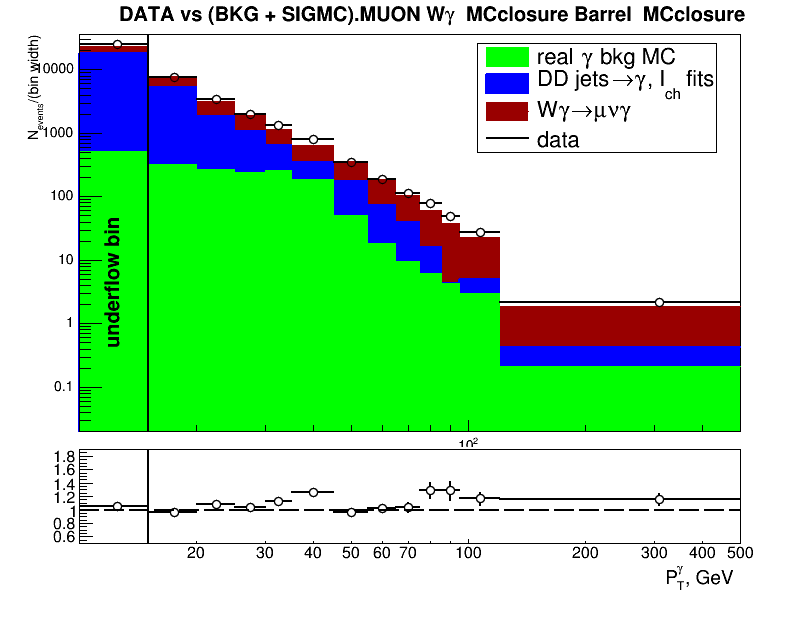
\includegraphics[width=0.33\textwidth]{../figs/figs_v11/MUON_WGamma/PrepareYields/c_DATAvsBkgPlusSigMCc_MUON_WGamma_TEMPL_CHISO_UNblind_MCclosure__Barrel__phoEt_MCclosure.png}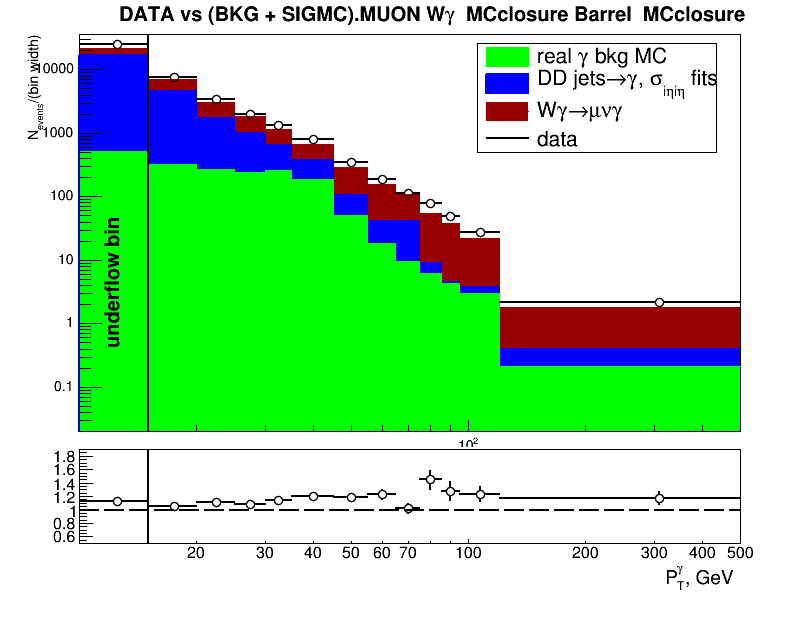
\includegraphics[width=0.33\textwidth]{../figs/figs_v11/MUON_WGamma/PrepareYields/c_DATAvsBkgPlusSigMCc_MUON_WGamma_TEMPL_SIHIH_UNblind_MCclosure__Barrel__phoEt_MCclosure.png}
  \caption{Left: data (top) and pseudodata (bottom) vs MC. Middle and right: data (top) and pseudodata (bottom) vs background estimates and signal MC in bins of $P_T^{\gamma}$. Jets$\rightarrow\gamma$ background estimated from fits of $I_{ch}^{\gamma}$ (middle) and  $\sigma_{i\eta i\eta}^{\gamma}$ (right). Muon channel. Barrel photons.}
  \label{fig:DATAvsBKGandSIGMC_MCclosure_MUON_B}
  \end{center}
\end{figure}

\begin{figure}[htb]
  \begin{center}
   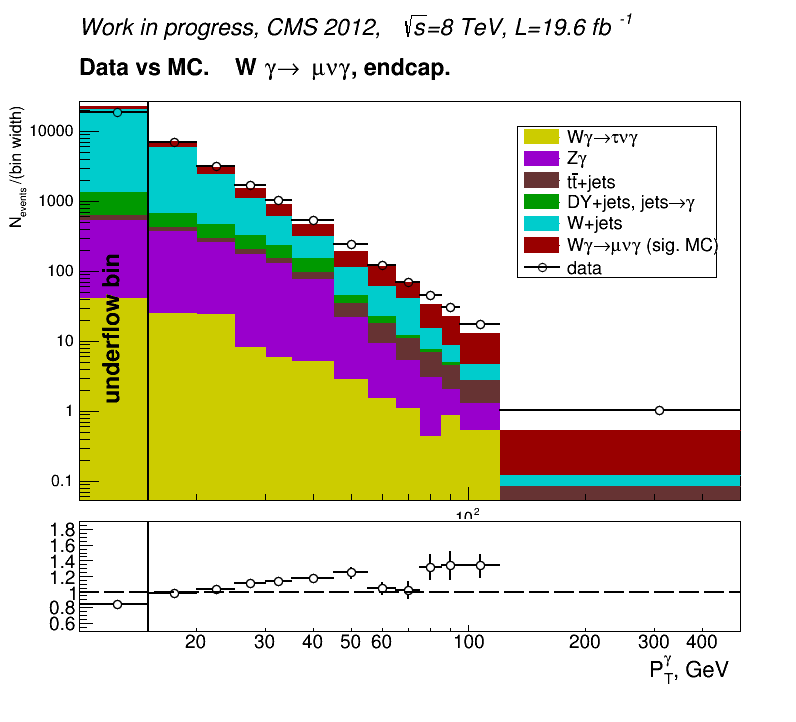
\includegraphics[width=0.33\textwidth]{../figs/figs_v11/MUON_WGamma/PrepareYields/c_TotalDATAvsMC_Endcap__phoEt.png}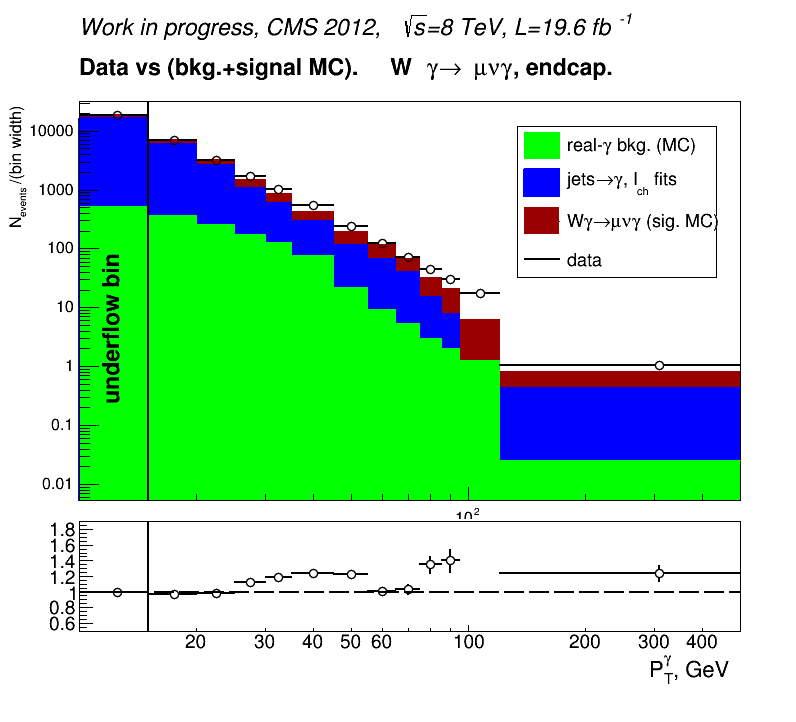
\includegraphics[width=0.33\textwidth]{../figs/figs_v11/MUON_WGamma/PrepareYields/c_DATAvsBkgPlusSigMCc_MUON_WGamma_TEMPL_CHISO_UNblind__Endcap__phoEt.png}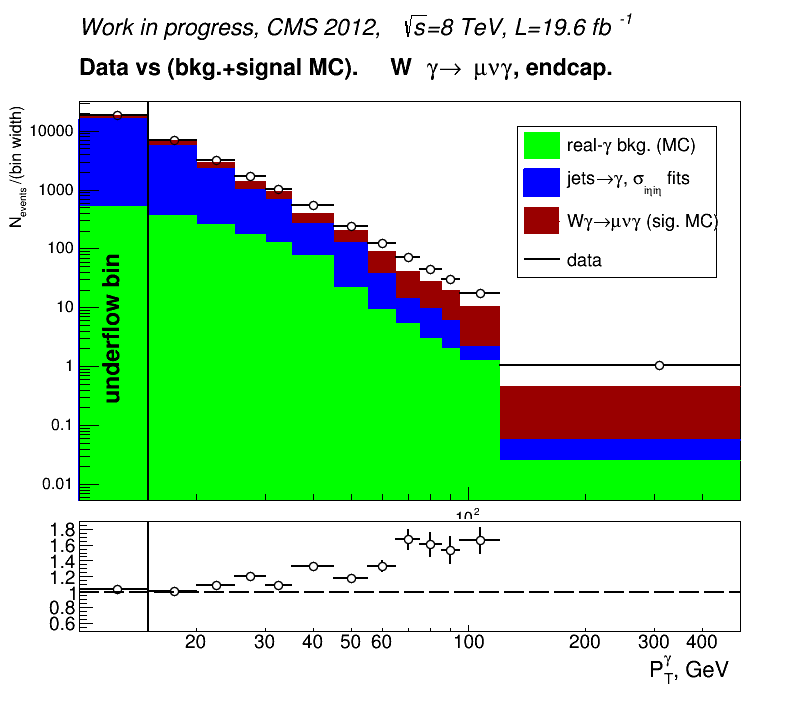
\includegraphics[width=0.33\textwidth]{../figs/figs_v11/MUON_WGamma/PrepareYields/c_DATAvsBkgPlusSigMCc_MUON_WGamma_TEMPL_SIHIH_UNblind__Endcap__phoEt.png}
   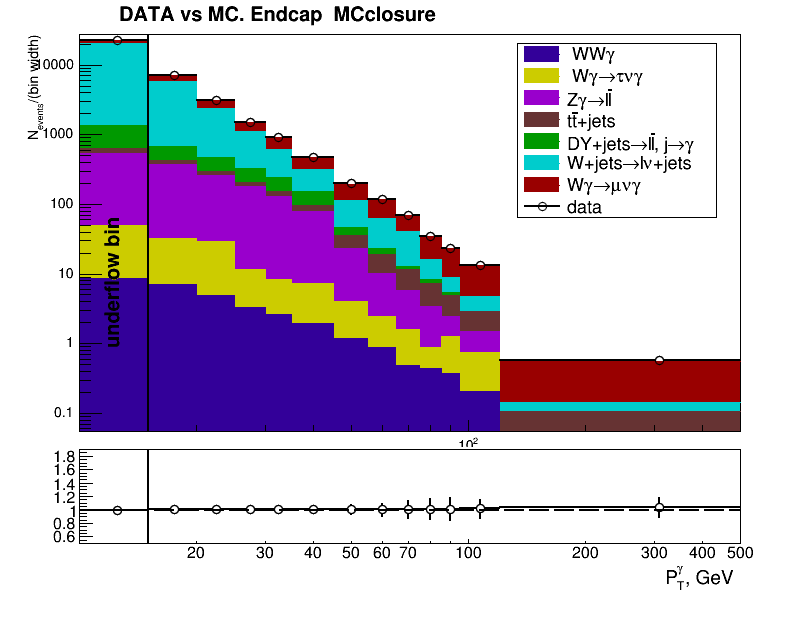
\includegraphics[width=0.33\textwidth]{../figs/figs_v11/MUON_WGamma/PrepareYields/c_TotalDATAvsMC_Endcap__phoEt_MCclosure.png}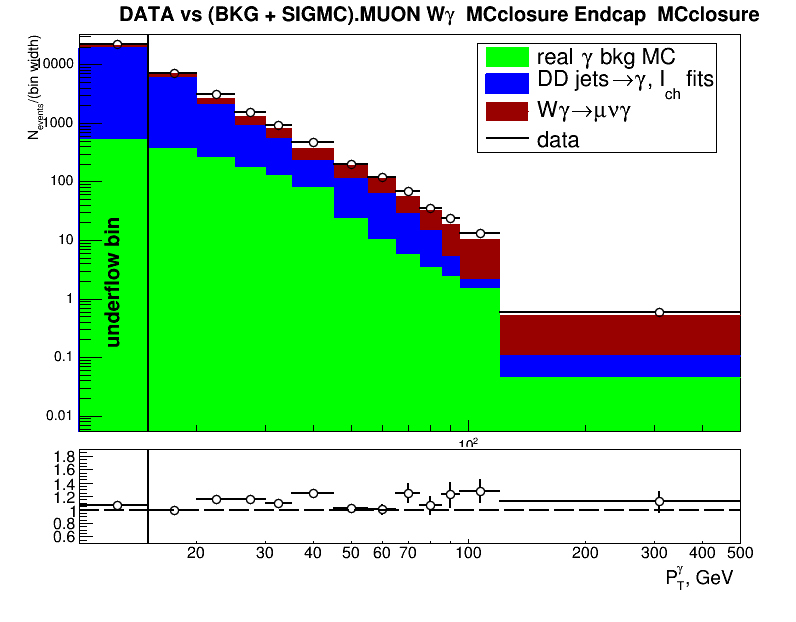
\includegraphics[width=0.33\textwidth]{../figs/figs_v11/MUON_WGamma/PrepareYields/c_DATAvsBkgPlusSigMCc_MUON_WGamma_TEMPL_CHISO_UNblind_MCclosure__Endcap__phoEt_MCclosure.png}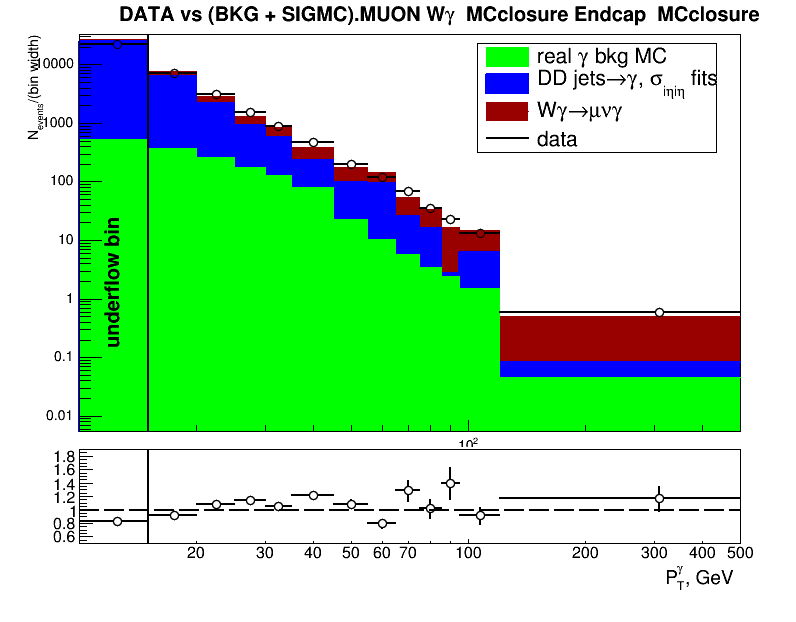
\includegraphics[width=0.33\textwidth]{../figs/figs_v11/MUON_WGamma/PrepareYields/c_DATAvsBkgPlusSigMCc_MUON_WGamma_TEMPL_SIHIH_UNblind_MCclosure__Endcap__phoEt_MCclosure.png}
  \caption{Left: data (top) and pseudodata (bottom) vs MC. Middle and right: data (top) and pseudodata (bottom) vs background estimates and signal MC in bins of $P_T^{\gamma}$. Jets$\rightarrow\gamma$ background estimated from fits of $I_{ch}^{\gamma}$ (middle) and  $\sigma_{i\eta i\eta}^{\gamma}$ (right). Muon channel. Endcap photons. }
  \label{fig:DATAvsBKGandSIGMC_MCclosure_MUON_E}
  \end{center}
\end{figure}

\begin{figure}[htb]
  \begin{center}
   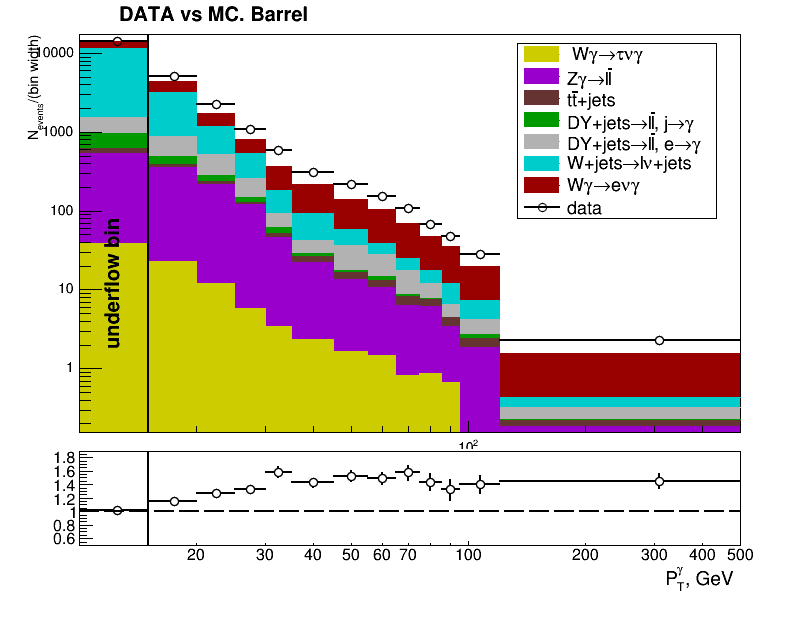
\includegraphics[width=0.33\textwidth]{../figs/figs_v11/ELECTRON_WGamma/PrepareYields/c_TotalDATAvsMC_Barrel__phoEt.png}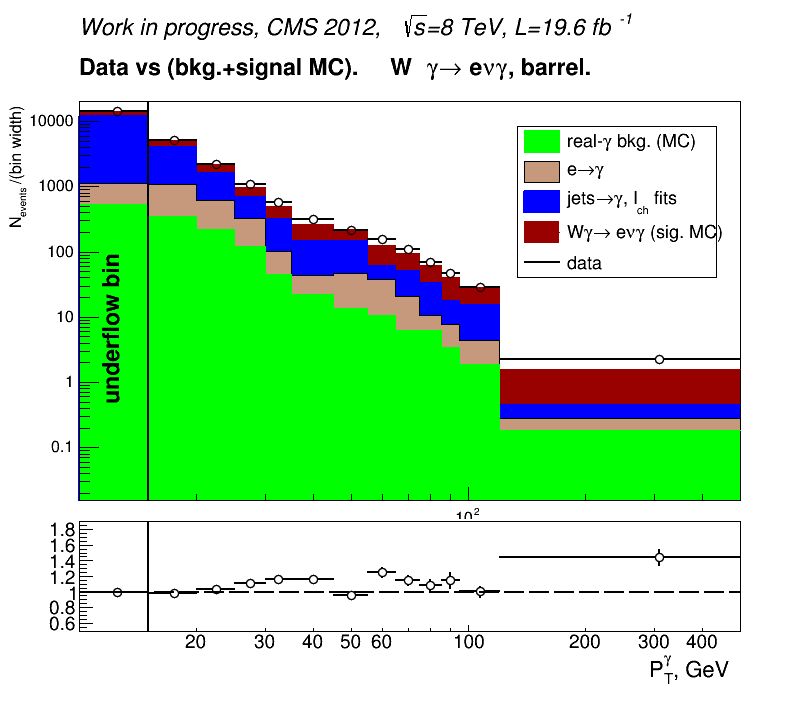
\includegraphics[width=0.33\textwidth]{../figs/figs_v11/ELECTRON_WGamma/PrepareYields/c_DATAvsBkgPlusSigMCc_ELECTRON_WGamma_TEMPL_CHISO_UNblind__Barrel__phoEt.png}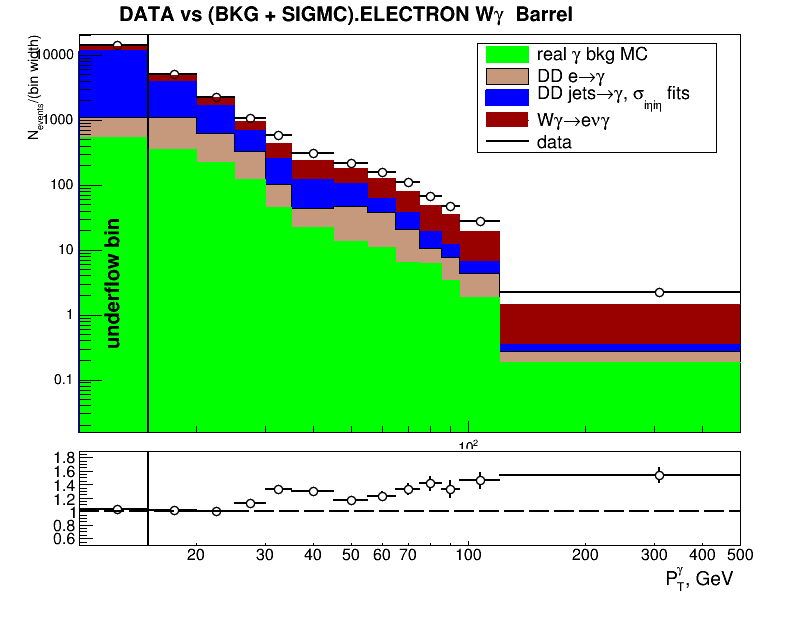
\includegraphics[width=0.33\textwidth]{../figs/figs_v11/ELECTRON_WGamma/PrepareYields/c_DATAvsBkgPlusSigMCc_ELECTRON_WGamma_TEMPL_SIHIH_UNblind__Barrel__phoEt.png}
   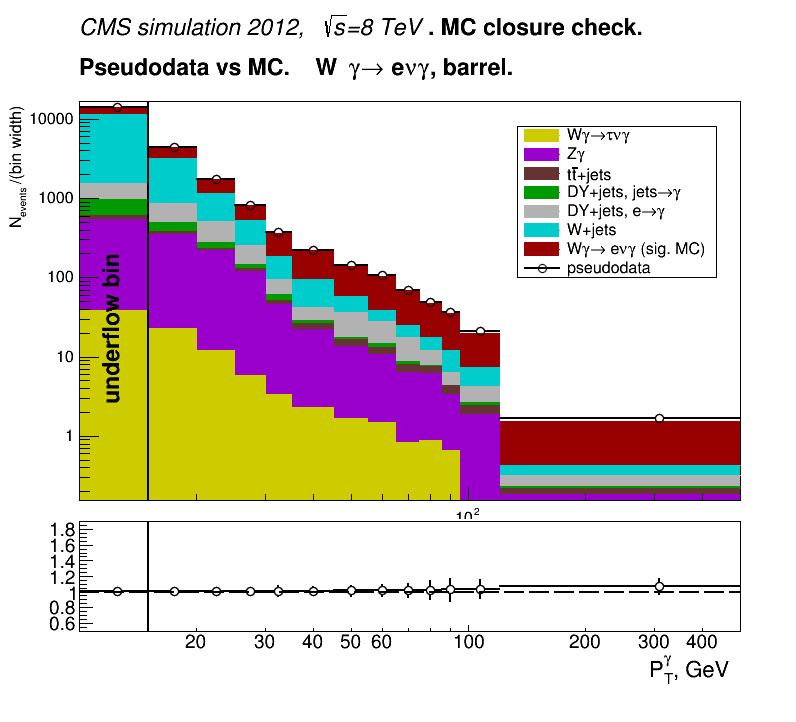
\includegraphics[width=0.33\textwidth]{../figs/figs_v11/ELECTRON_WGamma/PrepareYields/c_TotalDATAvsMC_Barrel__phoEt_MCclosure.png}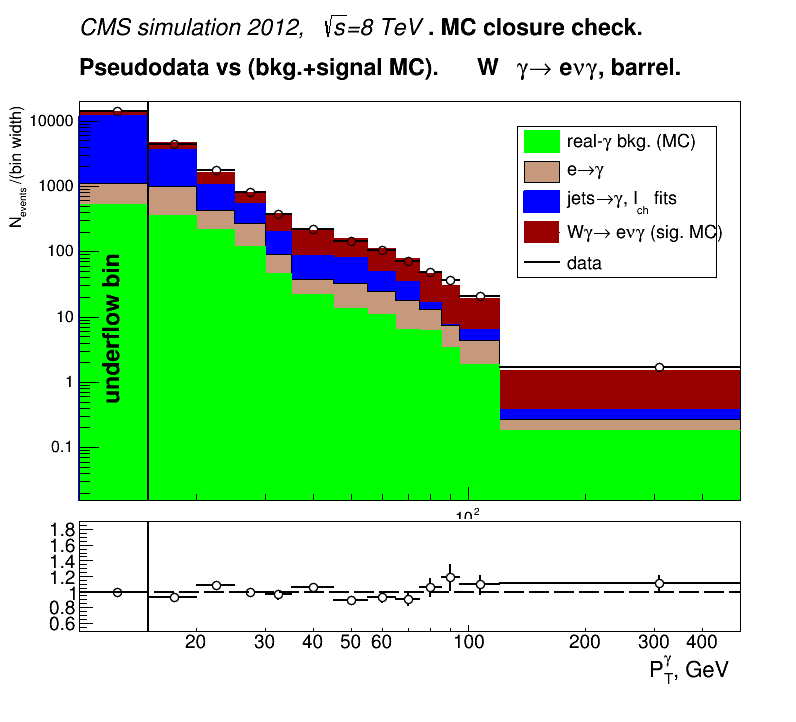
\includegraphics[width=0.33\textwidth]{../figs/figs_v11/ELECTRON_WGamma/PrepareYields/c_DATAvsBkgPlusSigMCc_ELECTRON_WGamma_TEMPL_CHISO_UNblind_MCclosure__Barrel__phoEt_MCclosure.png}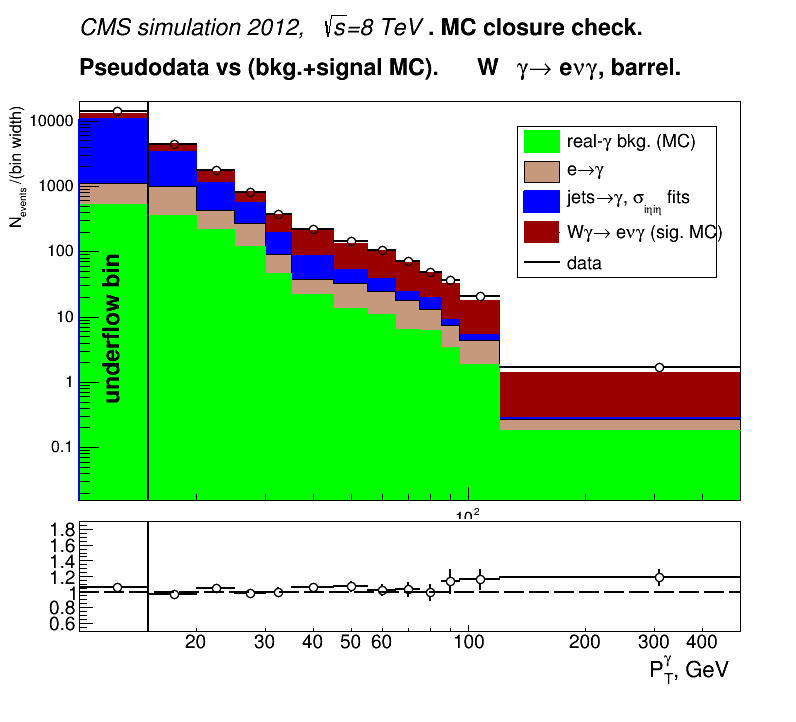
\includegraphics[width=0.33\textwidth]{../figs/figs_v11/ELECTRON_WGamma/PrepareYields/c_DATAvsBkgPlusSigMCc_ELECTRON_WGamma_TEMPL_SIHIH_UNblind_MCclosure__Barrel__phoEt_MCclosure.png}
  \caption{Left: data (top) and pseudodata (bottom) vs MC. Middle and right: data (top) and pseudodata (bottom) vs background estimates and signal MC in bins of $P_T^{\gamma}$. Jets$\rightarrow\gamma$ background estimated from fits of $I_{ch}^{\gamma}$ (middle) and  $\sigma_{i\eta i\eta}^{\gamma}$ (right). Electron channel. Barrel photons.}
  \label{fig:DATAvsBKGandSIGMC_MCclosure_ELECTRON_B}
  \end{center}
\end{figure}

\begin{figure}[htb]
  \begin{center}
   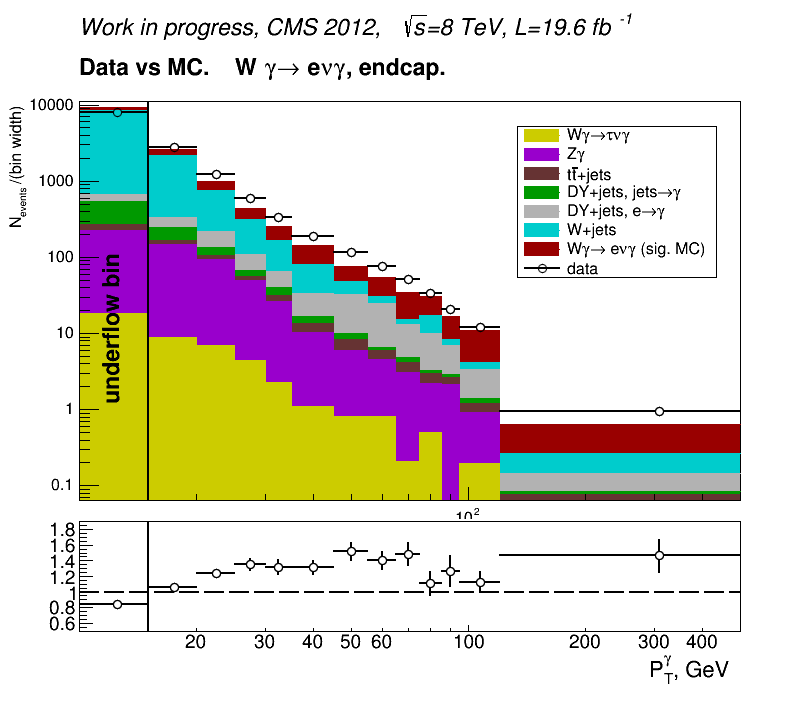
\includegraphics[width=0.33\textwidth]{../figs/figs_v11/ELECTRON_WGamma/PrepareYields/c_TotalDATAvsMC_Endcap__phoEt.png}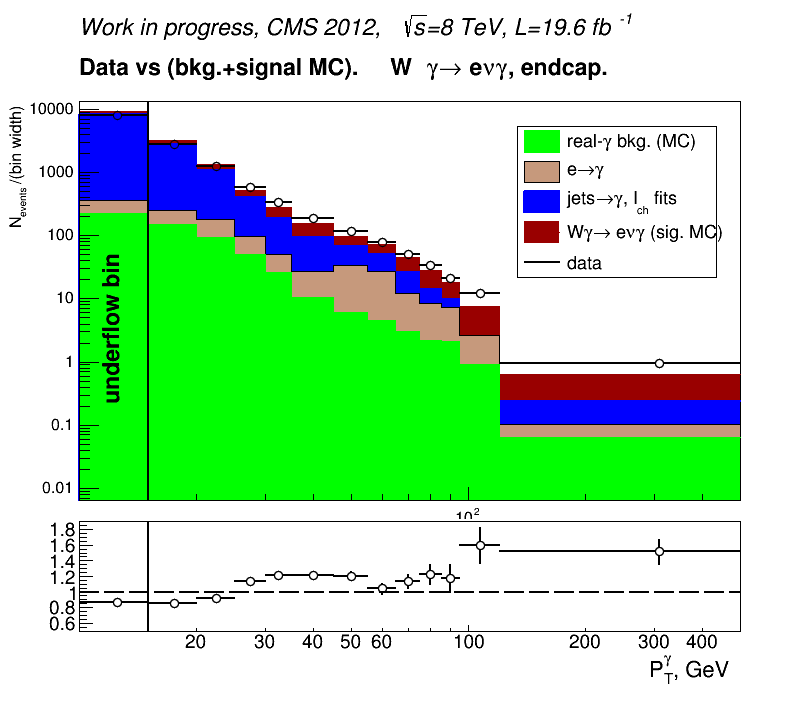
\includegraphics[width=0.33\textwidth]{../figs/figs_v11/ELECTRON_WGamma/PrepareYields/c_DATAvsBkgPlusSigMCc_ELECTRON_WGamma_TEMPL_CHISO_UNblind__Endcap__phoEt.png}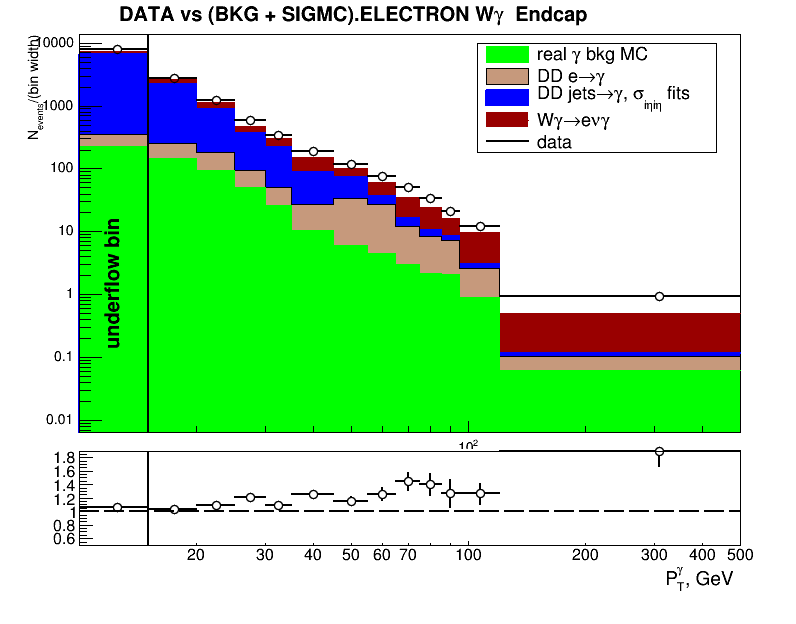
\includegraphics[width=0.33\textwidth]{../figs/figs_v11/ELECTRON_WGamma/PrepareYields/c_DATAvsBkgPlusSigMCc_ELECTRON_WGamma_TEMPL_SIHIH_UNblind__Endcap__phoEt.png}
   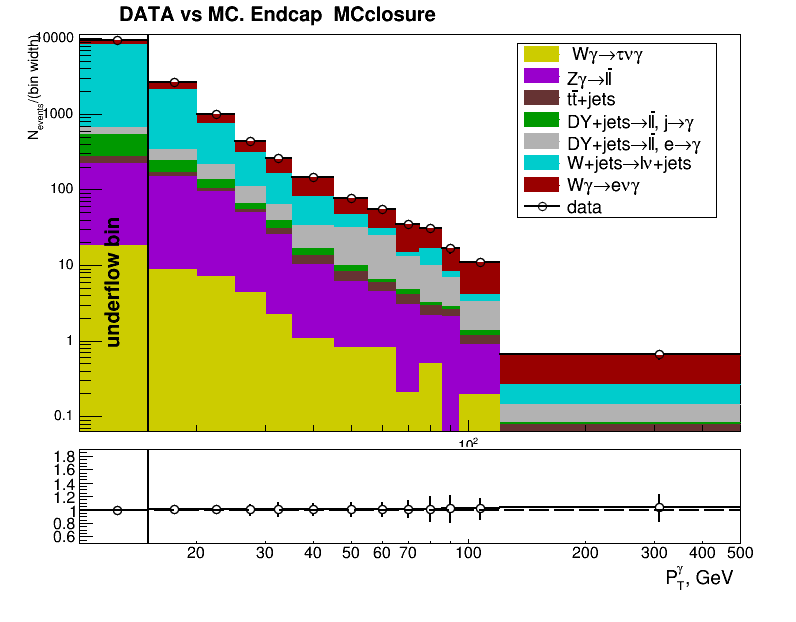
\includegraphics[width=0.33\textwidth]{../figs/figs_v11/ELECTRON_WGamma/PrepareYields/c_TotalDATAvsMC_Endcap__phoEt_MCclosure.png}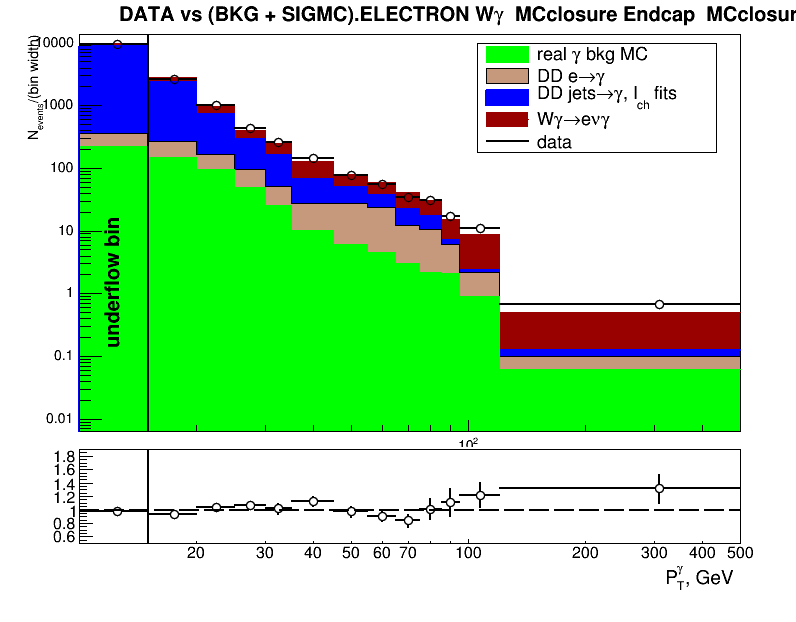
\includegraphics[width=0.33\textwidth]{../figs/figs_v11/ELECTRON_WGamma/PrepareYields/c_DATAvsBkgPlusSigMCc_ELECTRON_WGamma_TEMPL_CHISO_UNblind_MCclosure__Endcap__phoEt_MCclosure.png}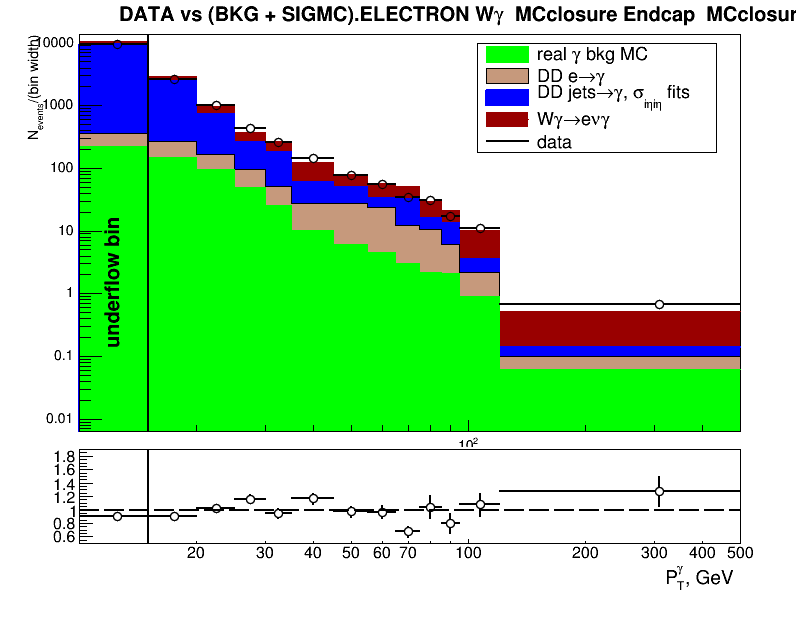
\includegraphics[width=0.33\textwidth]{../figs/figs_v11/ELECTRON_WGamma/PrepareYields/c_DATAvsBkgPlusSigMCc_ELECTRON_WGamma_TEMPL_SIHIH_UNblind_MCclosure__Endcap__phoEt_MCclosure.png}
  \caption{Left: data (top) and pseudodata (bottom) vs MC. Middle and right: data (top) and pseudodata (bottom) vs background estimates and signal MC in bins of $P_T^{\gamma}$. Jets$\rightarrow\gamma$ background estimated from fits of $I_{ch}^{\gamma}$ (middle) and  $\sigma_{i\eta i\eta}^{\gamma}$ (right). Electron channel. Endcap photons.}
  \label{fig:DATAvsBKGandSIGMC_MCclosure_ELECTRON_E}
  \end{center}
\end{figure}
